\chapter{Desenvolvimento}\label{cap_intro}

 Foram usadas as tecnologias de Java e Swing (código e telas) em conjunto com a IDE IntelliJ, Jena (framework para aplicações de web semântica) e GIT (gerenciamento de versão) para criação deste sistema. O atual escopo, apesar de diferente do proposto inicialmente (recomendação de lugares) prevê aplicar os mesmos conceitos com as mesmas tecnologias.

Essa mudança se deu devido a dificuldade de encontrar bases de dados coerentes e familiares contendo geolocalização, de forma a evitar a criação de uma pequena e experimental base optou-se pela utilização do tema filmes.

\section{Tela}

 A aplicação conta com uma única tela onde o usuário tem a liberdade de aplicar os filtros desejados a fim de obter uma recomendação.
 
 \subsection{Parâmetro Inicial} 
 
 Assim que é inicializada podemos observar (Figura 1) o primeiro campo para a pesquisa que conta com as opções: ''Actor'', ''Director'', ''Genre'' e ''Movie Name''. Ator, diretor, gênero e nome do filme, respectivamente (Figura 2).
 
 \begin{figure}[H]
 	\centering
 	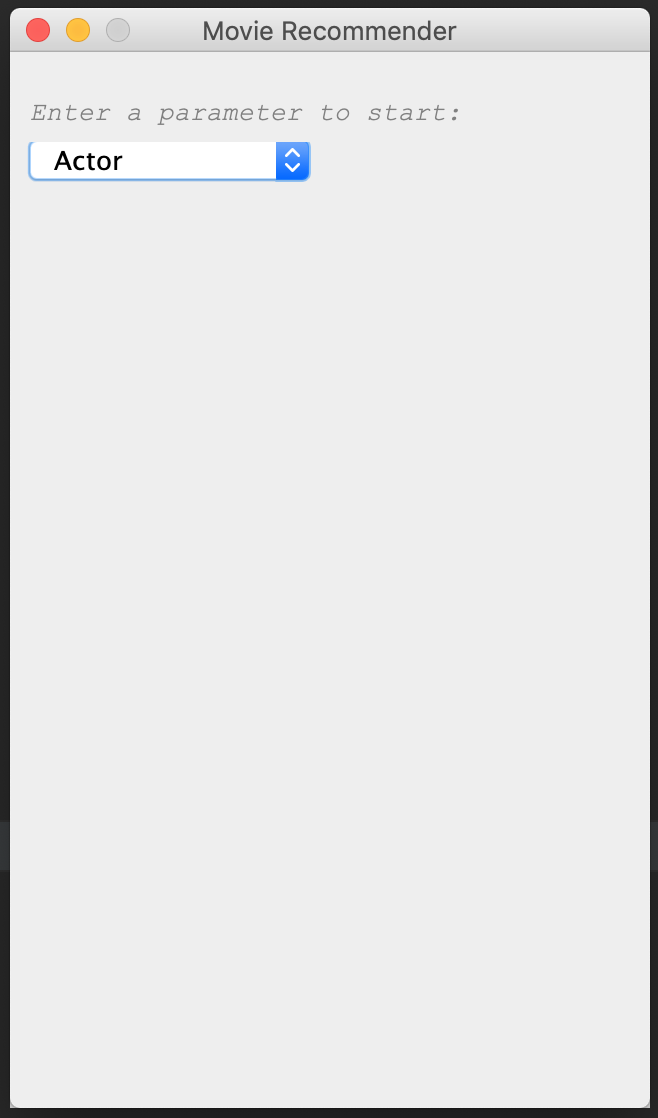
\includegraphics[width=0.5\linewidth]{images/telaInicial1}
 	\caption{Tela Inicial}
 	Fonte: pessoal.
 	\label{fig:Tela Inicial}
 \end{figure}
 
 \begin{figure}[H]
 	\centering
 	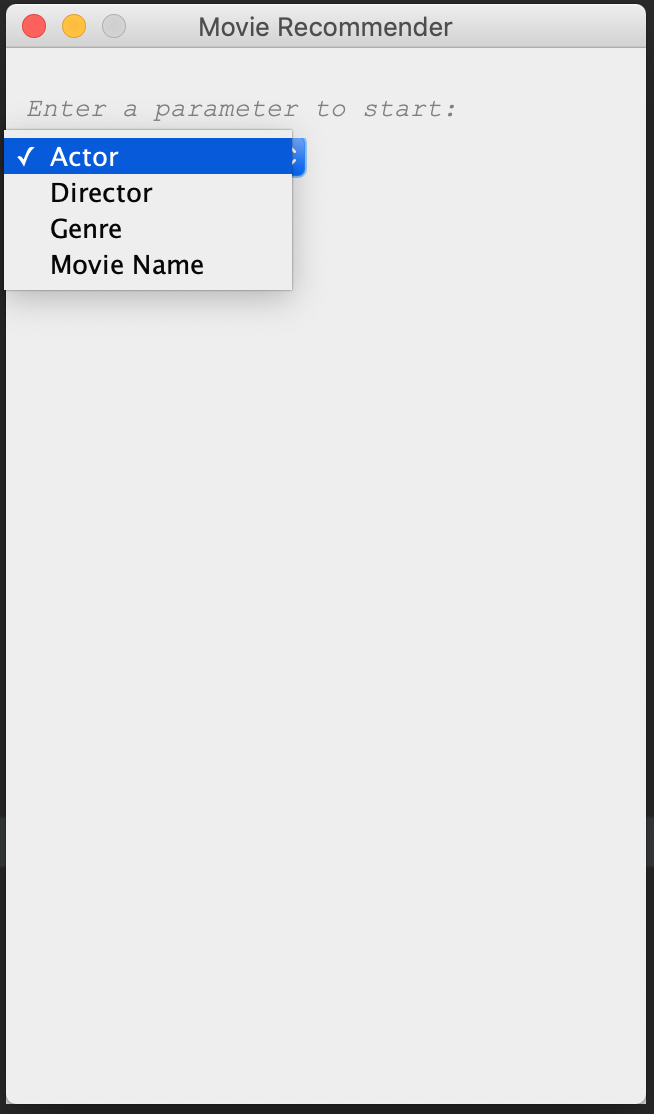
\includegraphics[width=0.5\linewidth]{images/telaInicial2}
 	\caption{Tela Inicial}
 	Fonte: pessoal.
 	\label{fig:Tela Inicial}
 \end{figure}

\subsection{Parâmetro de Entrada} 

 Tendo o usuário selecionado o primeiro parâmetro, é necessário informar o parâmetro de entrada que será usado na query para trazer as informações correspondentes.
 
 No exemplo (Figura 3), optou-se pelo parâmetro inicial ''Actor'' e parâmetro de entrada igual a ''Leonardo DiCaprio''.
 
  \begin{figure}[H]
 	\centering
 	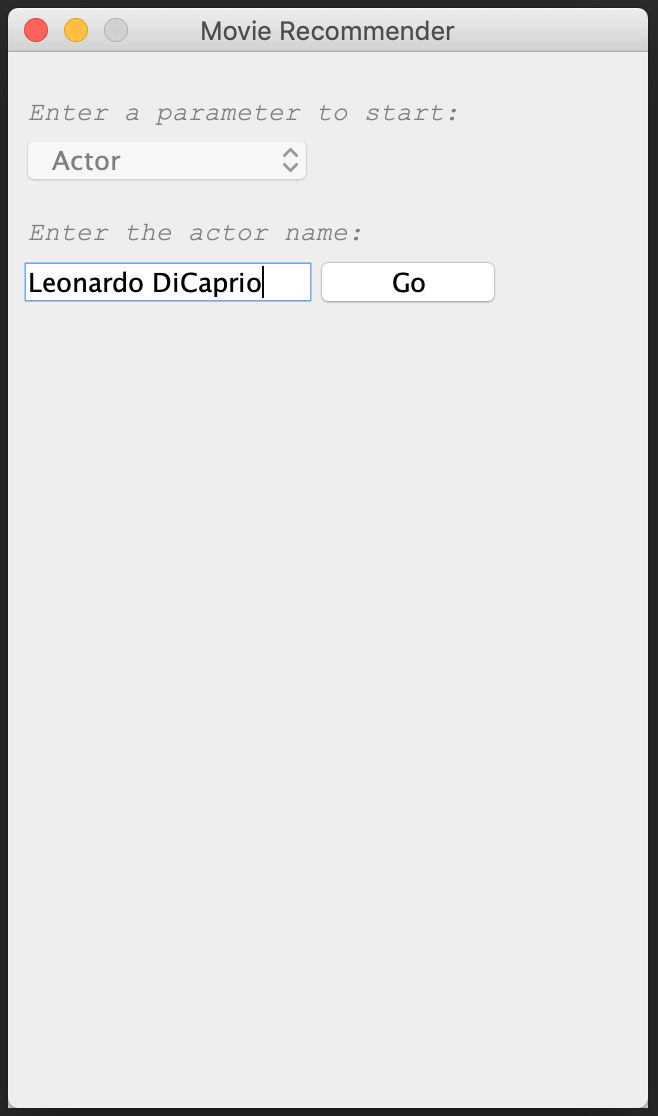
\includegraphics[width=0.5\linewidth]{images/telaInicialPreenchida}
 	\caption{Tela Inicial Preenchida}
 	Fonte: pessoal.
 	\label{fig:Tela Inicial Preenchida}
 \end{figure}

 Evidentemente, ao pressionar o botão ''Go'' a query será executada e as informações existentes na base de dados RDF serão trazidas para a tela em formato de recomendação (Figura 4).
 
   \begin{figure}[H]
 	\centering
 	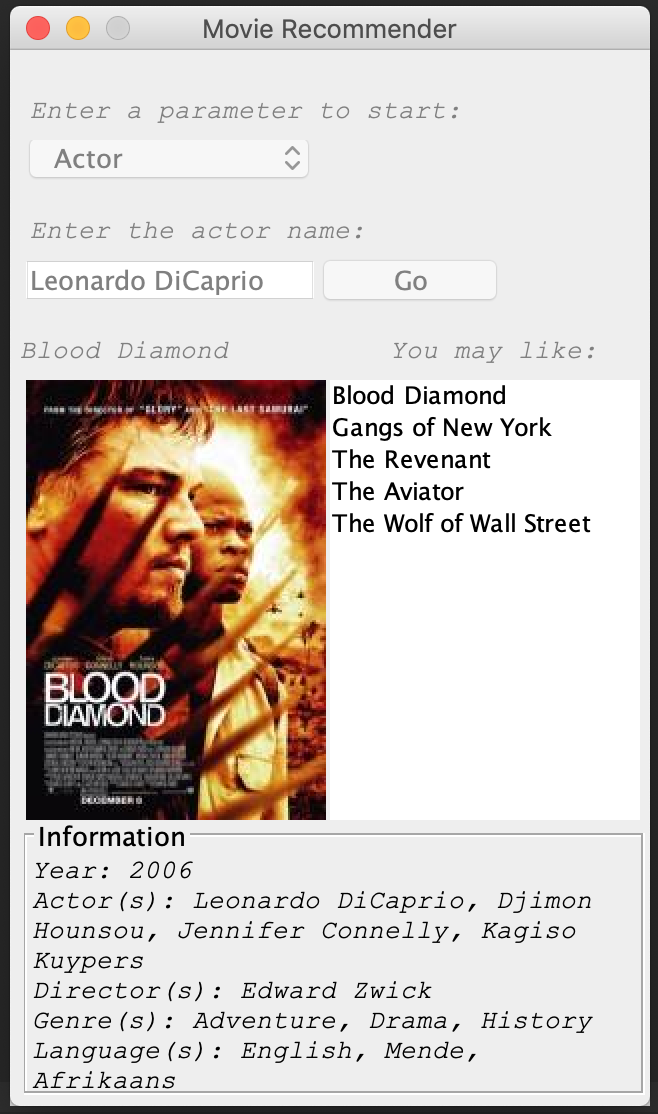
\includegraphics[width=0.5\linewidth]{images/telaInicialRecomendacao}
 	\caption{Tela Inicial com Recomendações}
 	Fonte: pessoal.
 	\label{fig:Tela Inicial com Recomendações}
 \end{figure}


\subsection{Funcionalidades e Navegação} 
 
 Uma vez que a pesquisa foi realizada com sucesso, o usuário encontra à esquerda o pôster, à direita as recomendações equivalentes aos parâmetros fornecidos e abaixo informações pertinentes ao filme.
 
 O usuário tem liberdade de escolher outro filme na sessão ''You may like'', alterando, evidentemente, as informações exibidas (Figura 5).
 
   \begin{figure}[H]
	\centering
	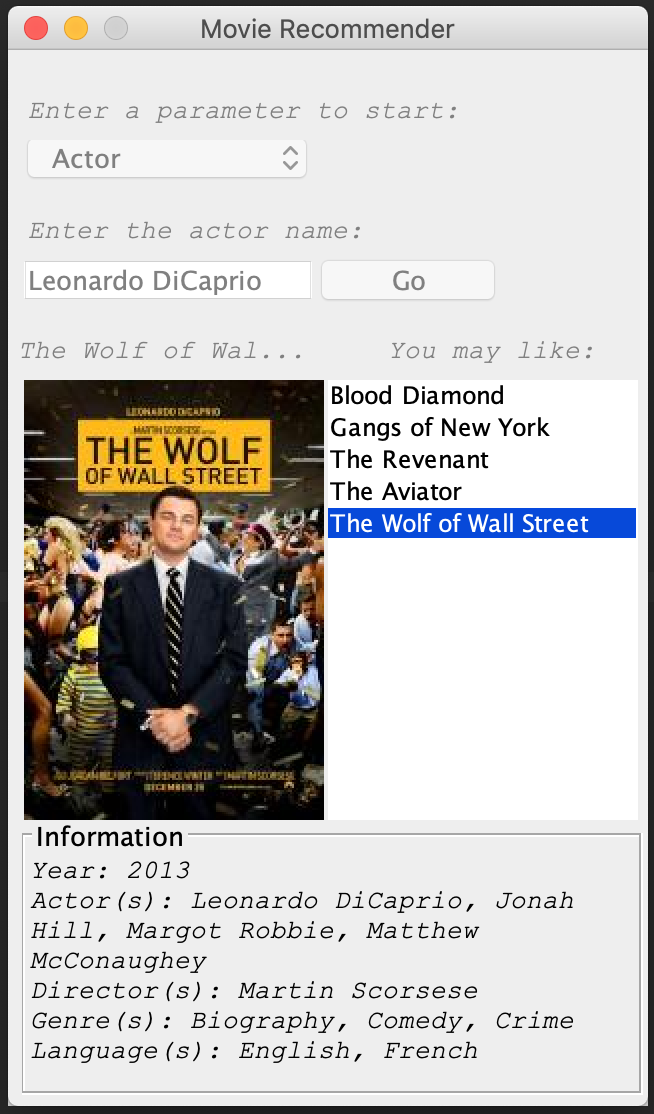
\includegraphics[width=0.5\linewidth]{images/telaInicialRecomendacao2}
	\caption{Tela Inicial alternando Recomendações}
	Fonte: pessoal.
	\label{fig:Tela Inicial alternando Recomendações}
\end{figure}
 
 A aplicação ainda prevê o encaminhamento para a crítica do filme pelo jornal estadunidense The New York Times, se existente, por intermédio do clique do mouse no pôster (Figura 6).
 
   \begin{figure}[H]
	\centering
	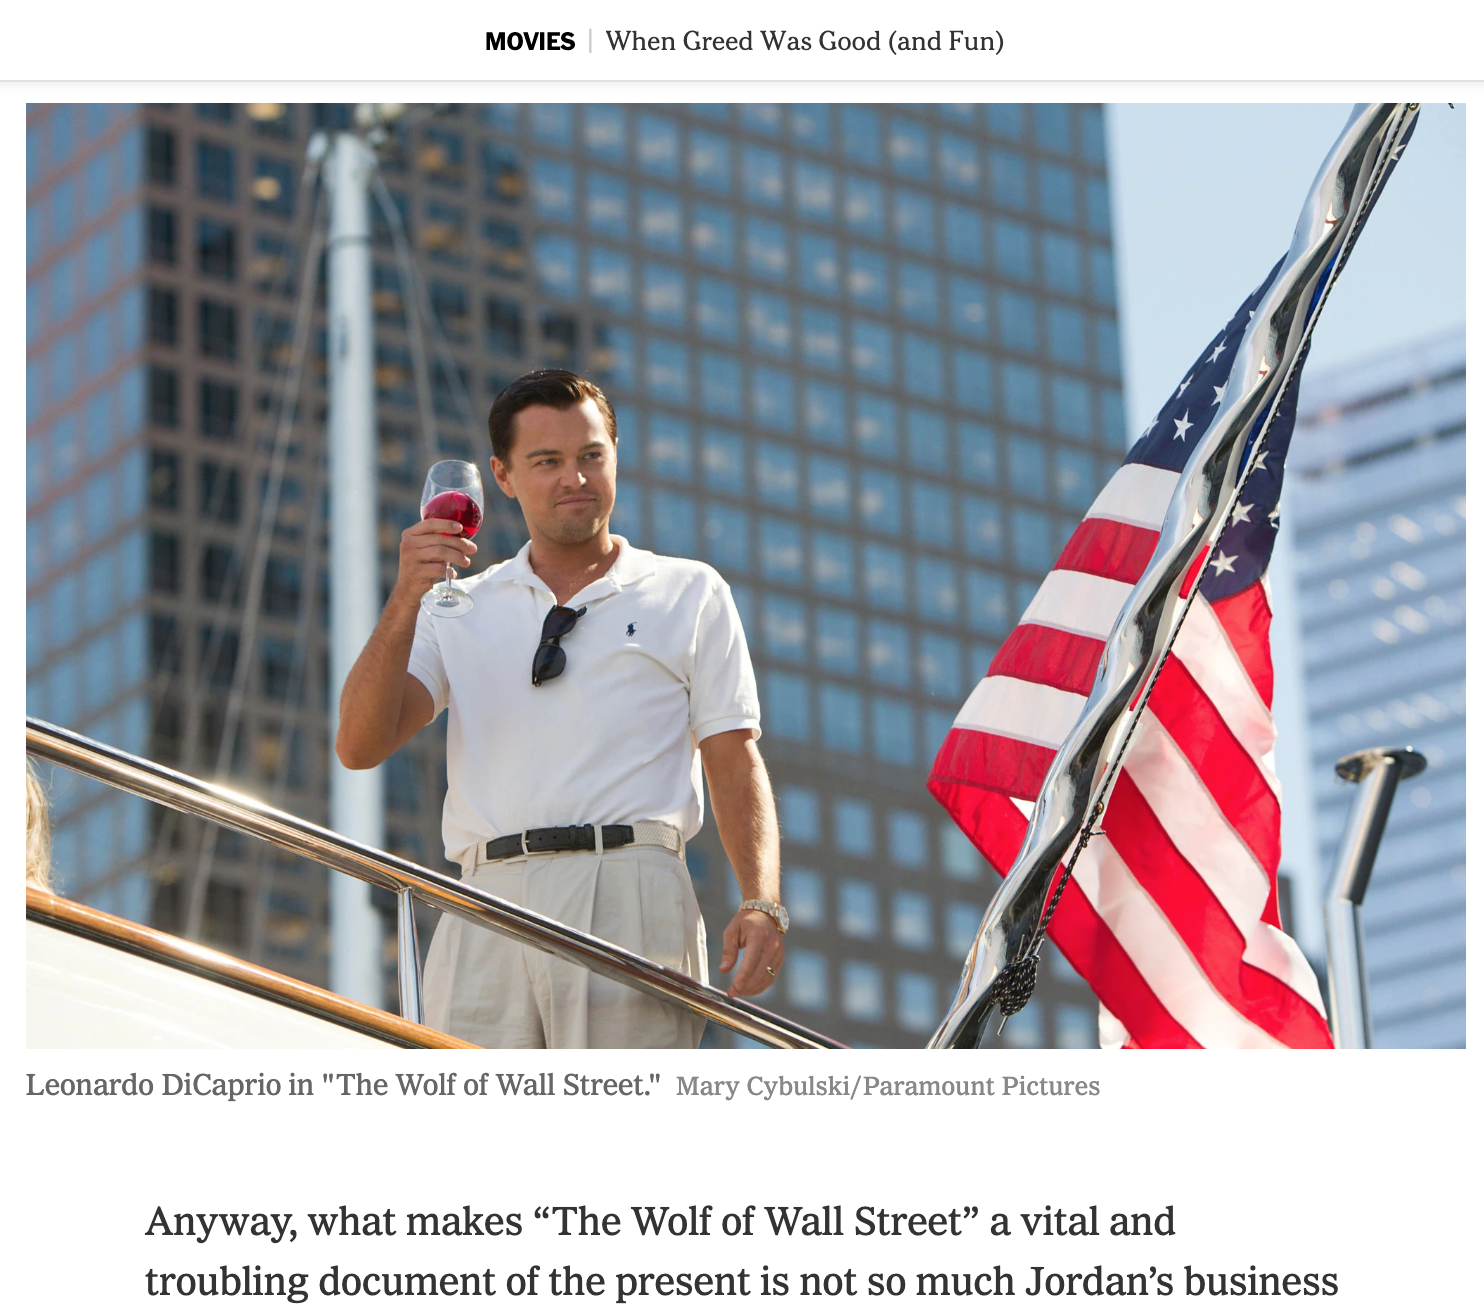
\includegraphics[width=0.6\linewidth]{images/NYTIMES}
	\caption{Crítica - The New York Times}
	Fonte: pessoal.
	\label{fig:Crítica - The New York Times}
\end{figure}

\section{Consulta/Query}

 As queries buscam, especificamente, o parâmetro de entrada baseado no parâmetro inicial.
 
 No exemplo anterior, utilizou-se o parâmetro inicial ''Actor'' e parâmetro de entrada ''Leonardo DiCaprio''. Dessa forma, a aplicação deve montar a querie seguindo o formato abaixo (Figura 7).

\begin{figure}[H]
	\centering
	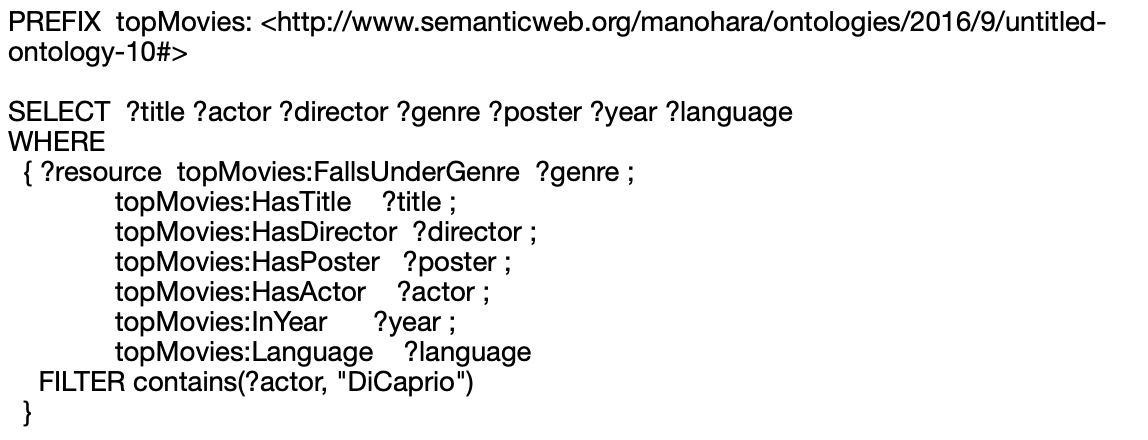
\includegraphics[width=0.8\linewidth]{images/Query}
	\caption{Exemplo de Query}
	Fonte: pessoal.
	\label{fig:Exemplo de Query}
\end{figure}

A manipulação é feita por intermédio da classe ResultSet do Java e permite a atribuição do resultado nas variáveis para exibição.